\chapter{Relazioni Ricorsive}

\begin{flushleft}
    Una successione $\{a_n\}_{n \in \mathbb{N}}$ a valori interi può essere data in due forme differenti:
    \begin{itemize}[nosep]
        \item per \textbf{elencazione}: $\{a_0, a_1, ..., a_i, ...\}$, con $a_i \in \mathbb{Z} \; \forall i \in \mathbb{N}_0$
        \item in \textbf{forma chiusa}: $a_n = f(n)$, con $f : \mathbb{N}_0 \mapsto \mathbb{Z}$, $f$ è un'\textbf{applicazione}
    \end{itemize}

    \textbf{Successioni Definite per Ricorsione}: una successione è definita \textbf{ricorsivamente} (ovvero tramite una \textbf{relazione ricorsiva}) se ogni termine della successione è espresso in funzione dei termini precedenti, e se sono noti un certo numero di termini iniziali che permettano di individuare univocamente la successione.

    Risolvere una \textit{relazione ricorsiva} significa ottenere una definizione in forma chiusa della successione stessa.

    \begin{boxA}
        \textcolor{orange}{\textbf{Esempio}} \\
        $\begin{cases}
            a_n = 3 \cdot a_{n - 1} \quad n > 1 \; \text{(relazione ricorsiva)} \\
            a_1 = 3 \qquad \qquad \qquad \;\; \text{(condizione iniziale)}
        \end{cases}$ \\
        definisce univocamente la successione \fcolorbox{orange}{white}{$\{a_n\}_{n \in \mathbb{N}} = \{3, 3^2, 3^3, ...\}$} che si può rappresentare in forma chiusa come:

        {\centering
            $a_n = 3^n \; \forall n \in \mathbb{N}$
        \par}
    \end{boxA}

    Una relazione ricorsiva si dice di \textbf{ordine \textit{k}} se il generico elemento $a_n$ della successione è dato in funzione di $k$ elementi che lo precedono. La relazione ricorsiva determinerà univocamente una successione, noti i $k$ elementi iniziali della successione

    Una relazione ricorsiva di ordine $k$ si dice \textbf{lineare} se viene rappresentata come:

    {\centering
        $a_n = b_{n - 1}(n) \cdot a_{n - 1} + b_{n - 2}(n) \cdot a_{n - 2} + ... + b_{n - k}(n) \cdot a_{n - k} + d(n)$
    \par}
    dove i $b_{n - i}(n) \; i \in \mathbb{N}$ sono delle funzioni (non necessariamente lineari) che determinano i coefficienti $a_{n - i} \; i \in \mathbb{N}$ mentre $d(n)$ è il termine noto (può non essere lineare).

    Una relazione ricorsiva \textit{lineare} si dice \textbf{omogenea} se il termine noto è nullo, ovvero $d(n) = 0$

    Una relazione ricorsiva \textit{lineare} si dice a \textbf{coefficienti costanti} se le funzioni coefficienti [$b_{n - i}(n) \; i \in \mathbb{N}$] sono funzioni costanti, ovvero $b_{n - i}(n) = \alpha_i$, con $\alpha_i$ costante $\forall i$ e viene rappresentata:

    {\centering
        $a_n = \alpha_1 \cdot a_{n - 1} + \alpha_2 \cdot a_{n - 2} + ... + \alpha_k \cdot a_{n - k} + d(n)$
    \par}
\end{flushleft}

\section{Relazioni Ricorsive Lineari del 1$^\circ$ Ordine}

\begin{flushleft}
    \textbf{Relazioni ricorsive lineari omogenee del I ordine a coefficienti costanti}: la successione definita da: 

    {\centering
        $\begin{cases}
            a_n = b \cdot a_{n - 1} \quad \forall n > m \\
            a_m = c
        \end{cases}$
    \par}
    ha come forma chiusa: \fcolorbox{red}{white}{$a_n = c \cdot b^{n - m} \; \forall n \geq m$}

    \begin{boxA}
        \textcolor{olive}{\textbf{Dimostrazione}}: si dimostra per \textbf{induzione} \newline
        \textcolor{red}{\textbf{Passo Iniziale}}: poniamo $n = m$ allora avremo che: 

        {\centering
            $a_n = c \cdot b^{m - m} = c \cdot b^0 = c$
        \par}
        abbiamo dimostrato le condizioni di partenza della relazione ricorsiva.

        \textcolor{red}{\textbf{Passo Induttivo}}

        {\centering
            \begin{minipage}[t]{0.45\textwidth}
                \centering
                \textbf{Hp.} $a_{n - 1} = c \cdot b^{n - 1 - m}$
            \end{minipage}
            \begin{minipage}[t]{0.45\textwidth}
                \centering
                \textbf{Th.} $a_n = c \cdot b^{n - m}$
            \end{minipage}
            $a_n = b \cdot a_{n - 1} = b \cdot c \cdot b^{n - 1 - m} = c \cdot b^{n - m}$
        \par}

        \textcolor{orange}{\textbf{Esempio}}

        {\centering
            $\begin{cases}
                a_n = 3a_{a - 1} \\
                a_0 = 2
            \end{cases}$
            $\Rightarrow a_n = 2 \cdot 3^{n - 0} = 2 \cdot 3^n$
        \par}
    \end{boxA}
    \textbf{Relazioni ricorsive lineari omogenee del I ordine a coefficienti non costanti}: la successione definita da:

    {\centering
        $\begin{cases}
            a_n = b(n) \cdot a_{n - 1} \quad \forall n > m \\
            a_m = c
        \end{cases}$
    \par}
    ha come forma chiusa \fcolorbox{red}{white}{$a_n = c \cdot \underset{i = 1}{\overset{n - m}{\prod}} b (m + i) \; \forall n \geq m$}. La forma chiusa può essere dimostrata per \textbf{induzione}, in perfetta analogia al caso precedente:
\end{flushleft}

\newpage
\begin{flushleft}

    \textbf{Relazioni ricorsive lineari del I ordine non omogenee a coefficienti costanti}: la successione definita da:

    {\centering
        $\begin{cases}
            a_n = b \cdot a_{n-1} + d(n) \quad \forall n > m \\
            a_m = c
        \end{cases}$
    \par}
    ha come forma chiusa: \fcolorbox{red}{white}{$a_n = b^{n-m} \cdot [c + \underset{i = 1}{\overset{n-m}{\sum}} d(m + i) \cdot b^{-i}] \; \forall n \geq m$}

    \begin{boxA}
        \textcolor{olive}{\textbf{Dimostrazione}}: la forma chiusa viene dimostrata sempre per \textbf{induzione}

        \textcolor{red}{\textbf{Passo Iniziale}}: poniamo $n = m$

        {\centering
            $a_n = b^{m-m} \cdot [c + \underset{i = 1}{\overset{m-m}{\sum}} d(m + i) \cdot b^{-i}] = [c + \cancel{\underset{i = 1}{\overset{0}{\sum}} d(m + i) \cdot b^{-1}}] = c$
        \par}

        \textcolor{red}{\textbf{Passo Induttivo}}

        {\centering
            \begin{minipage}[t]{0.45\textwidth}
                \centering
                \textbf{Hp.} \\
                $a_{n - 1} = b^{n-1-m} \cdot [c + \underset{i=1}{\overset{n-1-m}{\sum}} d(m + i) \cdot b^{-i}]$
            \end{minipage}
            \begin{minipage}[t]{0.45\textwidth}
                \centering
                \textbf{Th.} \\
                $a_n = b^{n-m} \cdot [c + \underset{i = 1}{\overset{n-m}{\sum}} d(m + i) \cdot b^{-i}]$
            \end{minipage}
        \par}

        $a_n = b \cdot a_{n-1} + d(n) = b \cdot b^{n-1-m} [c + \underset{i=1}{\overset{n-1-m}{\sum}} d(m+i) \cdot b^{-1}] + d(n) \cdot \fcolorbox{brown}{white}{$(b^{n-m} \cdot b^{-(n-m)})$}$ moltiplico e divido per $b^{n-m}$ in modo da poter raccogliere al primo addendo.
        \begin{align*}
            a_n &= b \cdot b^{n-1-m} [c + \underset{i=1}{\overset{n-1-m}{\sum}} d(m+i) \cdot b^{-1}] + d(n) \cdot (b^{n-m} \cdot b^{-(n-m)}) \\
            &= b^{n-m} [c + \underset{i=1}{\overset{n-1-m}{\sum}} d(m+i) \cdot b^{-1}] + d(n) \cdot (b^{n-m} \cdot b^{-(n-m)}) \\
            &= b^{n-m} \cdot \{[c + \underset{i=1}{\overset{n-1-m}{\sum}} d(m+i) \cdot b^{-1}] + \fcolorbox{blue}{white}{$d(n) \cdot b^{-(n-m)}$}\} \\
            &= b^{n-m} \cdot [c + \underset{i = 1}{\overset{n-m}{\sum}} d(m + i) \cdot b^{-i}]
        \end{align*}
        Il valore \fcolorbox{blue}{white}{$d(n) \cdot b^{-(n-m)}$} posso portarlo dentro alla sommatoria in modo da poter ottenere e dimostrare la tesi.
    \end{boxA}
\end{flushleft}

\begin{boxA}
    \textcolor{orange}{\textbf{Esempio - Torre di Hanoi}}: bisogna spostare $n$ dischi di diametro crescente, in modo da riottenere la torre sull'ultima colonna. \textbf{Regole}: ad ogni passo si può spostare un solo disco, un disco non può mai essere spostato sopra ad uno di diametro inferiore.
    
    \begin{center}
        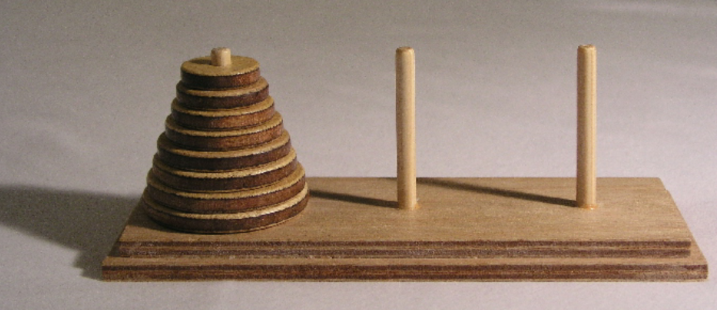
\includegraphics[width=0.65\textwidth]{img/hanoi}
    \end{center}

    Per spostare il generico $n$-esimo disco: $H_n = H_{n-1} + 1 + H_{n-1} = 2 \cdot H_{n-1} + 1$. Quindi la nostra relazione ricorsiva sarà:
    $H(n) = \begin{cases}
        H_n = 2 \cdot H_{n-1} + 1 \\
        H_1 = 1
    \end{cases}$
    
    \begin{align*}
        H(n) &= 2^{n-1} [1 + \underset{i=1}{\overset{n-1}{\sum}}1 \cdot 2^{-i}] \\
        &= 2^{n-1} [\underset{i=0}{\overset{n-1}{\sum}}1 \cdot 2^{-i}] \\
        &= 2^{n-1} \cdot \frac{1-(\frac{1}{2})^n}{1-\frac{1}{2}} \\
        &= 2^n \cdot (1 - \frac{1}{2^n}) = 2^n - 1 \; \text{mosse}
    \end{align*}
\end{boxA}

\begin{flushleft}
    \textbf{Relazioni ricorsive lineri non omogenee del I ordine a coefficienti non costanti}: la successione definita da:

    {\centering
        $\begin{cases}
            a_n = b(n) \cdot a_{n-1} + d(n) \quad \forall n > m \\
            a_m = c
        \end{cases}$
    \par}
    ha come forma chiusa: \fcolorbox{red}{white}{$a_n = \underset{i=1}{\overset{n-m}{\prod}} b(m+i) \cdot [c + \underset{i=1}{\overset{n-m}{\sum}} d(m+i) \cdot \underset{j=1}{\overset{i}{\prod}} \frac{1}{b(m+j)}] \; \forall n \geq m$}. La forma chiusa può essere verificata per \textbf{induzione} come il caso a \textit{coefficienti costanti}.
\end{flushleft}

\newpage
\section{Relazioni Ricorsive Lineari del 2 Ordine}
\begin{flushleft}
    \textbf{Algoritmi ``dividi et impera''}
    La decomposizione di un problema complesso in due o più sottoproblemi ricorsivi rappresenta un approccio molto efficace per la risoluzione di vari problemi computazionali, in informatica, permettendo di parallelizzare la computazione.

    \textbf{Relazioni ricorsive del tipo \textit{divide et impera}} \\
    La generica relazione ricorsiva che divide il problema in $k$ sottoproblemi (con $k \in \mathbb{N}$) è:

    {\centering
        $\begin{cases}
            s_n = b \cdot s_{\frac{n}{k}} + d(n) \quad \forall n > m \\
            s_m = c
        \end{cases}$
    \par}
    Si può supporre che $\exists z \in \mathbb{N}$ tale che $n = k^z$, ovvero $\log_k n = z$, possiamo esprimere la relazione ricorsiva come:

    {\centering
        $s_{k^z} = b \cdot s_{\frac{k^z}{k}} + d(k^z) = b \cdot s_{k^{z-1}} + d(k^z)$
    \par}

    Definiamo $s_{k^z} = r_z$, poniamo $d(k^z) = d'(z)$ e $\log_k m = m'$ otteniamo la relazione ricorsiva del tipo:

    {\centering
        $\begin{cases}
            r_z = b \cdot r_{z-1} + d'(z) \quad \forall z > m' \\
            r_{m'} = c
        \end{cases}$
    \par}
    Dalla soluzione in forma chiusa di tale \textit{relazione ricorsiva lineare non omogenea del I ordine}, si ricava infine la forma chiusa di $s_n$, applicando ad $r_z$ la sostituzione inversa: $r_z = s_n$ e $z = \log_k n$.
    \begin{boxA}
        \textcolor{orange}{\textbf{Esempio: Ricerca Binaria}} \\
        Data una lista ordinata di $n$ elementi, per cercarne uno non è necessario dover scorrere tutta la lista, basta confrontare l'elemento a metà, dividendo quindi il problema in due sotto-problemi. 

        {\centering
            $\begin{cases}
                c_n = 1 + c_{\frac{n}{2}} \quad \forall n > 1 \\
                c_1 = 1 \qquad \qquad \text{se ho solo un elemento dovrò fare un solo confronto}
            \end{cases}$
        \par}
        Supponendo $n = 2^z$ (ovvero $z = \log_2 n$) e ponenedo $c_n = c_{2^z} = r_z$ otteniamo:

        {\centering
            $\begin{cases}
                r_z = 1 + r_{z-1} \quad \forall n > m \\
                r_{\log_2 1} = r_0 = 1
            \end{cases}$
        \par}
        Allora la soluzione di questa relazione ricorsiva è: 
        
        {\centering
            \fcolorbox{orange}{white}{$r_z = b^{z-m} \cdot [c + \sum_{i=1}^{z-m} d'(m+i) \cdot b^{-i}] = 1 + \sum_{i=1}^z \ = 1 + z$}
        \par}
        Sostituendo $z = \log_2 n$ otteniamo il valore di $r_{\log_2 n} = c_{2^{\log_2 n}} = c_n$ quindi otteniamo: 
        
        {\centering
            \fcolorbox{red}{white}{$c_n = 1 + \log_2 n$}
        \par}
        
    \end{boxA}
\end{flushleft}

\newpage
\begin{flushleft}
    \textbf{Relazioni ricorsive lineari omogenee del II ordine a coefficienti costanti}: è univocamente determinata, $\forall n \geq m$, la successione $a_n$ tale che: 

    {\centering
        $\begin{cases}
            a_n = \alpha_1 \cdot a_{n-1} + \alpha_2 \cdot a_{n-1} \quad \forall n > m + 1\\
            a_m = c_1 \\
            a_{m+1} = c_2
        \end{cases}$
    \par}

    \textcolor{blue}{\textbf{Lemma A}}: data la relazione ricorsiva $a_n = \alpha_1 \cdot a_{n-1} + \alpha_2 \cdot a_{n-2}$, se $a'_n$ e $a''_n$ sono due successione che la verificano, allora $\forall A, B \in \mathbb{C}$ andche la successione $a_n = A \cdot a'_n + B \cdot a''_n$ verifica la relazione ricorsiva data.
    \begin{boxA}
        \textcolor{olive}{\textbf{Dimostrazione}}

        {\centering
            \begin{minipage}[t]{0.45\textwidth}
                \centering
                \textbf{Hp.} \\
                $a'_n = \alpha_1 \cdot a'_{n-1} + \alpha_2 \cdot a'_{n-2}$ \\
                $a''_n= \alpha_1 \cdot a''_{n-1} + \alpha_2 \cdot a''_{n-2}$
            \end{minipage}
            \hfill
            \begin{minipage}[t]{0.45\textwidth}
                \centering
                \textbf{Th.} \\
                $a_n = \alpha_1 \cdot a_{n-1} + \alpha_2 \cdot a_{n-2}$ \\
                $\forall A, B \in \mathbb{C} \; \text{t.c.} \; a_n = A \cdot a'_n + B \cdot a''_n$
            \end{minipage}
        \par}
        \begin{align*}
            \alpha_1 \cdot a_{n-1} + \alpha_2 \cdot a_{n-2} &= \alpha_1(A \cdot a'_{n-1} + B \cdot a''_{n-1}) + \alpha_2(A \cdot a'_{n-2} + B \cdot a''_{n-2}) \\
            &= A(\alpha_1 \cdot a'_{n-1} + \alpha_2 \cdot a'_{n-2}) + B (\alpha_1 \cdot a''_{n-1} + \alpha_2 \cdot a''_{n-2}) \\
            &= A \cdot a'_n + B \cdot a''_n \quad \text{|| è la nostra tesi}
        \end{align*}
    \end{boxA}
    \textcolor{blue}{\textbf{Lemma B}}: data la relazione ricorsiva $a_n = \alpha_1 \cdot a_{n-1} + \alpha_2 \cdot a_{n-2}$, la successione $a_n = r^n, \; r \neq 0$ è soluzione di tale relazione ricorsiva se e solo se $r$ è radice dell'equazione (\textbf{equazione caratteristica della rel. ric.}): $x^2 - \alpha_1 x - \alpha_2 = 0$
    \begin{boxA}
        \textcolor{olive}{\textbf{Dimostrazione}}: essendo un \textit{se e solo se} bisogna dimostrare entrambi i casi. \newline
        \textcolor{red}{\textbf{Prima Parte}}: ``$\Rightarrow$'' 

        {\centering
            \begin{minipage}[t]{0.45\textwidth}
                \centering
                \textbf{Hp.} $r \neq 0$ è soluzione dell'equazione caratteristica $x^2 - \alpha_1 x - \alpha_2 = 0$ \\
            \end{minipage}
            \hfill
            \begin{minipage}[t]{0.45\textwidth}
                \centering
                \textbf{Th.} $a_n = r^n$ verifica la relazione ricorsiva $a_n = \alpha_1a_{n-1} + \alpha_2a_{n-2}$ \\
            \end{minipage}
        \par}
        
        \begin{flushleft}
            Per \textbf{Hp.} abbiamo $r^2 - \alpha_1r - \alpha_2 = 0$, moltiplico per $r^{n-2}$ (siccome $r \neq 0$ posso farlo) e ottengo $r^n - \alpha_1r^{n-1} - \alpha_2r^{n-2} = 0$, ma a questo punto $a_n = r^n$ che verifica la relazione ricorsiva e quindi la nostra tesi.
        \end{flushleft}
        \textcolor{red}{\textbf{Seconda Parte}} ``$\Leftarrow$''

        {\centering
            \begin{minipage}[t]{0.45\textwidth}
                \centering
                \textbf{Th.} $a_n = r^n$ verifica la relazione ricorsiva $a_n = \alpha_1a_{n-1} + \alpha_2a_{n-2}$ \\
            \end{minipage}
            \hfill
            \begin{minipage}[t]{0.45\textwidth}
                \centering
                \textbf{Hp.} $r$ è soluzione dell'equazione caratteristica $x^2 - \alpha_1 x - \alpha_2 = 0$ \\
            \end{minipage}
        \par}
        \begin{flushleft}
            Per \textbf{Hp.}: $r^n = \alpha_1r^{n-1} + \alpha_2r^{n-2}$ portando tutto al primo membro e dividendo per $r^{n-2}$ ottengo $r^2 - \alpha_1r - \alpha_2 = 0$ ovvero $r$ è soluzione dell'equazione caratteristica.
        \end{flushleft}
    \end{boxA}

    \newpage
    \textcolor{blue}{\textbf{Lemma C}}: data

    {\centering
        $\begin{cases}
            a_n = \alpha_1 \cdot a_{n-1} + \alpha_2 \cdot a_{n-2} \quad \forall n > m + 1 \\
            a_m = c_1 \\
            a_{m+1} = c_2
        \end{cases}$
    \par}
    se l'equazione caratteristica della relazione ricorsiva ammette due radici distinte $r_1, r_2 \neq 0$, allora l'unica soluzione della relazione ricorsiva che verifica le condizioni iniziali date è del tipo 
    
    {\centering
        \fcolorbox{red}{white}{$a_n = A \cdot r_1^n + B \cdot r_2^n \; \text{con} \; A, B \in \mathbb{C}$}
    \par}
    \begin{boxA}
        \textcolor{olive}{\textbf{Dimostrazione}} \\
        \textbf{Hp.} | l'equazione caratteristica $x^2 -\alpha_1x - \alpha_2 = 0$ ha $\Delta \neq 0$ ($r_1, r_2 \neq$ distinte) \\
        \textbf{Th.} | l'unica successione che verifica la relazione ricorsiva: 

        {\centering
            $\begin{cases}
                a_n = \alpha_1 \cdot a_{n-1} + \alpha_2 \cdot a_{n-2} \quad \forall n > m + 1 \\
                a_m = c_1 \\
                a_{m+1} = c_2
            \end{cases}$
        \par}
        è del tipo \fcolorbox{violet}{white}{$a_n = \overline{A} \cdot r_1^n + \overline{B} \cdot r_2^n$} con $\overline{A}, \overline{B} \in \mathbb{C}$

        Per il \textcolor{blue}{lemma B}, sia $a'_n = (r_1)^n$ che $a''_n = (r_2)^n$ verificano la relazione ricorsiva, ma allora, per il \textcolor{blue}{lemma A}, ogni successione $a_n = A(r_1)^n è B(r_2)^n$ verifica la relazione ricorsiva.

        Dobbiamo quindi cercare se una di queste successioni verifica anche le condizioni iniziali. Imponiamo quindi:
        
        {\centering
            $\begin{cases}    
                \;\;\; (a_m =)A(r_1)^m + (r_2)^m = c_1 \\
                (a_{m+1} =)A(r_1)^{m+1} + (r_2)^{m_+1} = c_2
            \end{cases}$
        \par}
        Questo è un sistema di due equazioni a due incoglite con una matrice dei coefficenti:

        {\centering
        $M = \left(\begin{array}{cc} (r_1)^m & (r_2)^m \\
            (r_1)^{m+1} & (r_2)^{m+1} \end{array}\right)$
        \par}
        Andiamo a calcolarci ora il \textit{determinante} $\det(M) = (r_1)^m \cdot (r_2)^{m+1} - (r_1)^{m+1} \cdot (r_2)^m$ ovvero:

        {\centering
            $\det(M) = (r_1r_2)^m(r_2-r_1) \neq 0 \; \Rightarrow \; \rho(M) = 2$
        \par}
        Il sistema è un sistema di Cramer, quindi $\exists ! Sol(\overline{A}, \overline{B})$.
    \end{boxA}

    \newpage
    \textcolor{blue}{\textbf{Lemma D}}: data la relazione ricorsiva $a_n = \alpha_1 \cdot a_{n-1} + \alpha_2 \cdot a_{n-2}$, se l'equazione caratteristica presenta due radici $r$ coincidenti e non nulle, allora anche la successione $a''_n = n \cdot r^n$ verifica la relazione ricorsiva.
    \begin{boxA}
        \textcolor{olive}{\textbf{Dimostrazione}}

        {\centering
            \begin{minipage}[t]{0.45\textwidth}
                \centering
                \textbf{Hp.} l'equazione caratteristica $x^2-\alpha_1x-\alpha_2 = 0$ ha $\Delta = 0$
            \end{minipage}
            \hfill
            \begin{minipage}[t]{0.45\textwidth}
                \centering
                \textbf{Th.} la successione $a_n = n \cdot r^n$ verifica la relazione ricorsiva $a_n = \alpha_1a_{n-1} + \alpha_2a_{n-2}$
            \end{minipage}
        \par}
        
        \begin{flushleft}
            Per \textbf{Hp.} abbiamo che $x^2 - \alpha_1x - \alpha_2 = (x-r)^2 = x^2 - 2rx + r^2$ quindi avremo che $\alpha_1 = 2r$ mentre $\alpha_2 = r^2$ e quindi la relazione ricorsiva sarà: $a_n = 2ra_{n-1} - r^2a_{n-2}$.

            Dobbiamo ora verificare che $a''_n = n \cdot r^n$ verifichi la relazione ricorsiva: 
            \begin{align*}
                a''_n &= 2ra''_{n-1} - r^2a''_{n-2} \\
                &= 2r(n-1) \cdot r^{n-1} - r^2(n-2) \cdot r^{n-2} \\
                &= r^n[2(n-1) - (n-2)] \\
                &= r^n(2n - \cancel{2} - n + \cancel{2}) = n \cdot r^n
            \end{align*}
        \end{flushleft}
    \end{boxA}
    \textcolor{blue}{\textbf{Lemma E}}: data

    {\centering
        $\begin{cases}
            a_n = \alpha_1 \cdot a_{n-1} + \alpha_2 \cdot a_{n-2} \quad \forall n > m + 1 \\
            a_m = c_1 \\
            a_{m+1} = c_2
        \end{cases}$
    \par}
    se l'equazione caratteristica della relazione ricorsiva ammette due radici $r$ coincidenti e non nulle, allora l'unica soluzione della relazione ricorsiva che verifica le condizioni iniziali date è del tipo $a_n = A \cdot r^n + B \cdot n \cdot r^n, \; \text{con} \; A, B \in \mathbb{C}$
    \begin{boxA}
        \textcolor{olive}{\textbf{Dimostrazione}}:

        {\centering
            \begin{minipage}[t]{0.25\textwidth}
                \textbf{Hp.} l'eq. caratteristica $x^2-\alpha_1x-\alpha_2 = 0$ ha $\Delta = 0$
            \end{minipage}
            \hfill
            \begin{minipage}[t]{0.65\textwidth}
                \textbf{Th.} l'unica successione che verifica $\begin{cases} 
                    a_n = \alpha_1a_{n_1} + \alpha_2a_{n-2} \\
                    a_m = c_1 \\
                    a_{m+1} = c_2
                \end{cases}$ \\
                è del tipo $a_n = \overline{A} \cdot r^n + \overline{B} \cdot n \cdot r^n $ ($\overline{A}, \overline{B} \in \mathbb{C})$
            \end{minipage}
        \par}
        Per il \textcolor{blue}{lemma B}, $a'_n = r^n$ verifica la rel. ric., ma per il \textcolor{blue}{lemma D} anche $a''_n = nr^2$ la verifica. Quindi per il \textcolor{blue}{lemma A}, ogni successione $a_n = A \cdot r^n + B \cdot n \cdot r^n$ verifica la rel. ric. Imponiamo le confizioni iniziali:

        {\centering
            $\begin{cases}
                \;\;\; (a_m =)A \cdot r^m + B \cdot mr^m = c_1 \\
                (a_{m+1} =)A \cdot r^{m+1} + B (m+1) \cdot r^{m+1}
            \end{cases} \; \rightarrow \; M = \left(\begin{array}{cc} r^m & mr^m \\ r^{m+1} & (m+1) r^{m+1} \end{array}\right)$
        \par}
        Calcoliamo il determinante della matrice dei coefficenti:
        
        {\centering
            $\det(M) = r^m(m+1)r^{m+1} - r^{m+1}mr^m = r^{2m+1}(m+1) - r^{2m+1}m = r^{2m+1} \Rightarrow \exists ! Sol(\overline{A}, \overline{B})$
        \par}
    \end{boxA}
\end{flushleft}

\begin{flushleft}
    \textcolor{orange}{\textbf{Esercizio}}: supponendo che al primo mese si formi una coppia di conigli, che nel secondo mese diventi adulta e che nel terzo mese si generi una nuova coppia avremmo:

    {\centering
        $\begin{cases}
            F_n = F_{n-1} + F_{n-1} \quad \forall n > 1 \; \rightarrow \; \text{\textbf{successione di Fibonacci}} \\
            F_0 = 0 \\
            F_1 = 1
        \end{cases}$
    \par}
    Ricaviamo l'equazione caratteristica della relazione ricorsiva: $x^2-x-1 = 0$ che avrà radici pari a $r_{1,2} = \frac{1 \pm \sqrt{5}}{2}$. Per il \textcolor{blue}{lemma C}, la soluzione che verifica la relazione ricorsiva e le condizioni iniziali date è del tipo: $F_n = A \cdot r_1^n + B \cdot r_2^n$. Imponendo le condizioni iniziali avremmo:

    {\centering
        $\begin{cases}
            F_0 = 0 = A + B \\
            F_1 = 1 = A \cdot \frac{1 + \sqrt{5}}{2} + B \cdot \frac{1-\sqrt{5}}{2}
        \end{cases}
        \rightarrow
        \begin{cases}
            A = \frac{1}{\sqrt{5}} \\
            B = - \frac{1}{\sqrt{5}}
        \end{cases}$
    \par}
    La soluzione in forma chiusa è quindi: \fcolorbox{red}{white}{$F_n = \frac{1}{\sqrt{5}}(\frac{1+\sqrt{5}}{2})^n - \frac{1}{\sqrt{5}}(\frac{1-\sqrt{5}}{2})^2$}
    In particolare, $r_1 = \frac{1+\sqrt{5}}{2} = \phi$ è detto \textbf{sezione aurea}. Questo numero è molto importante in quanto indica il rapporto tra i lati dei rettangoli ``belli'', viene infatti utilizzato nell'arte, nell'estetica, etc... 

    Dagli esempi di utilizzo della sezione aure sono le carte di credito, le proporzioni dell'uomo vitruviano o le colonne partenopee

    \textbf{Proprietà della successione di Fibonacci - Paradosso di Lewis Carrol}: è possibile scomporre un quadrato di lato 8, per poi ricomporlo in un rettangolo di lati 5 e 13.
    
    \begin{figure}[h]
        \centering
        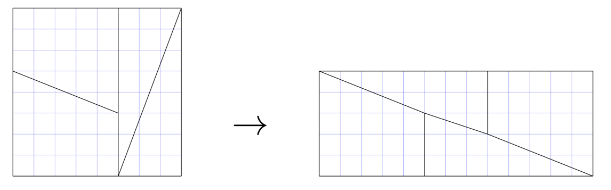
\includegraphics[width=0.45\textwidth]{img/fibonacci}
    \end{figure}
    \textbf{Identità di Cassini}: se $F_n$ denota l'$n$.esimo numeri di Fibonacci, allora: 

    {\centering
        $F_{n+1} \cdot F_{n-1} - F_n^2 = (-1)^n$
    \par}
    \begin{boxA}
        \textcolor{olive}{\textbf{Dimostrazione}}: si procedeper \textbf{induzione}. Per $n=1$ è banalmente vera, perché $1 \cdot 0 - (1)^2 = (-1)^1$. Supponiamo che l'identità valga per $n-1$ ovvero: $F_n \cdot F_{n-1} - F_{n-1}^2 = (-1)^{n-1}$ [ $F_n = F_{n-1} + F_{n-2} \; \rightarrow \; F_{n-2} = F_n - F_{n-1}$ ]
        \begin{align*}
            F_n \cdot (F_n - F_{n-1}) - F_{n-1}^2 &= (-1)^{n-1} \\
            (F_n)^2 - (F_n \cdot F_{n-1}) -F_{n-1}^2 &= (-1)^{n-1} \\
            (F_n)^2 - F_{n-1} \cdot (F_n + F_{n-1}) &= (-1)^{n-1}
        \end{align*}
        Poiche $F_n + F_{n-1} = F_{n+1}$ si ottiene l'identità di cassini per $n$: $F_n^2 - F_{n-1} \cdot F_{n+1} = (-1)^{n-1}$
    \end{boxA}
\end{flushleft}

\section{Relazioni Ricorsive Lineari di Ordine Superiore al 2}

\begin{flushleft}
    \textbf{Relazioni ricorsive lineari omogenee di ordin $k$ a coefficienti costanti}: è univocamente determinata, $\forall n \geq m$, la successione $a_n$ tale che:

    {\centering
        $\begin{cases}
            a_n = \alpha_1 a_{n-1} + \alpha_2 a_{n-2} + ... + a_k a_{n-1} \quad \forall n \geq m + k \\
            a_m = c_1 \\
            a_{m+1} = c_2 \\
            \vdots \\
            a_{m+k+1} = c_k 
        \end{cases}$
    \par}

    Dividiamo il \textbf{procedimento risolutivo} in step:
    \begin{enumerate}[nosep]
        \item si risolve l'\textit{equazione caratteristica} (di grado $k$):

        {\centering
            $x^k - \alpha_1 x^{k-1} - \alpha_2 x^{k-2} - ... - \alpha_k = 0$
        \par}
        questa soluzione ha sicuramente $k$ radici complesse, se ogni radice si considera con la sua molteplicità.
        \item per ogni radice $r$ di molteplicità $s$, si considerano le successioni: \\
        $a'_n = r^n$ \\
        $a''_n = n \cdot r^n$
        $a'''_n = n^2 \cdot r^n$
        $\vdots$ \\
        $a_n^{(s)} = n^{s-1} \cdot r^n$
        \item tutte e $k$ le successioni ottenute, sommate, verificheranno la relazione ricorsiva.
        \item imponendo le condizioni iniziali si ottiene un sistema di Cramer da cui si ottiene l'unica soluzioni
    \end{enumerate}
    \textbf{N.B.} il problema ``grosso'' in questi esercizi sarà il calcolo delle radici dell'equazione caratteristica (bisognerà utilizzare la scomposizione di \textbf{Ruffini})

    \begin{boxA}
        \textcolor{orange}{\textbf{Esercizio}} \\
        $\begin{cases}
            a_n = 10a_{n-1} - 33a_{n-2} + 36a_{n-3} \quad \forall n \geq 3 \\
            a_0 = 1 \\
            a_1 = 5 \\
            a_2 = 20
        \end{cases}$
        \begin{enumerate}[nosep]
            \item eq. caratteristica: $x^3 - 10x^2 + 33x - 36 = 0$, devo trovare le sue radici: $(x-3)^2(x-4) = 0$
            \item abbiamo trovato: $r_1 = 3$ con molteplicità 2, mentre $r_2 = 4$ con molteplicità 1
            \item ottenendo: $A \cdot 3^n + B \cdot n \cdot 3^n + C \cdot 4^n$
            \item impongo le condizion iniziali: \\
            $\begin{cases}
                (a_0 =) A \cdot 3^0 + B \cdot 0 \cdot 3^0 + C \cdot 4^0 = 1 \\
                (a_1 =) A \cdot 3^1 + B \cdot 1 \cdot 3^1 + C \cdot 4^1 = 5 \\
                (a_2 =) A \cdot 3^2 + B \cdot 2 \cdot 3^2 + C \cdot 4^2 = 20
            \end{cases}
            \rightarrow
            \begin{cases}
                A + C = 1 \\
                3A + 3B + 4C = 5 \\
                9A + 18B + 16C = 20
            \end{cases}$ \\
            $\begin{cases}
                A = 1 - C \\
                3 - 3C + 3B + 4C = 5 \\
                9 - 9C + 18B + 16C = 20
            \end{cases}
            \rightarrow
            \begin{cases}
                A = 1 - C \\
                3B + C = 2 \\
                18B + 7C = 11
            \end{cases}
            \rightarrow
            \begin{cases}
                A = 2 \\
                C = -1 \\
                B = 1
            \end{cases}$ \\
            Ottenendo \fcolorbox{red}{white}{$a_n = 2 \cdot 3^n + n \cdot 3^n - 4^n$}
        \end{enumerate}
    \end{boxA}
    
    \textbf{Relazioni ricorsive lineari non omogenee di ordine $k$}: è univocamente determinata, $\forall n \geq m$, la successione $a_n$ tale che:
    
    {\centering
        $\begin{cases}
            a_n = \alpha_1 \cdot a_{n-1} + \alpha_2 \cdot a_{n-2} + ... + \alpha_k \cdot a_{n-k} + d(n) \quad \forall n \geq m+k \\
            a_m = c_1 \\
            a_{m+1} = c_2 \\
            \vdots \\
            a_{m+k-1} = c_k
        \end{cases}$
    \par}
    È possibile verificare che le \textbf{soluzioni} di una relazione lineare ricorsiva non omogenea si ottengano: 
    \begin{itemize}[nosep]
        \item una soluzione della relazione ricorsiva non omogenea.
        \item tutte le soluzioni della relazione ricorsiva omogenea associata.
    \end{itemize}
    Non ci sono metodi generali per il calcolo della soluzione particolare della non omogenea, abbiamo un teorema per 2 casi particolari:
    
    \newpage
    \textbf{Teorema}: sia $d(n)$ il termine noto di una relazione ricorsiva lineare data.
    \begin{itemize}[nosep]
        \item sia $d(n) = c \cdot q^n$, con $c$ costante e $q \neq 0$. Se $q$ non è radice dell'equazione caratteristica, allora esiste una soluzione particolare del tipo $a_n = \beta \cdot q^n$. Se $q$ è radice dell'equazione caratteristica di molteplicità $s$, allora esiste una soluzione particolare del tipo $a_n = \beta \cdot n^s \cdot q^n$.
        \item sia $d(n)$ un polinomio in $n$ di grado $r$. Se 1 non è radice dell'equazione caratteristica del tipo $a_n = \beta_0 + \beta_1 \cdot n + ... + \beta_r \cdot n^r$. Se 1 è radice dell'equazione caratteristica di molteplicità $s$, esiste una soluzione particolare del tipo: $a_n = n^s \cdot (\beta_0 + \beta_1 \cdot n + ... + \beta_r \cdot n^r)$
    \end{itemize}
    \textbf{Corollario}: se il termine noto di una relazione ricorsiva lineare data è costante, allora:
    \begin{itemize}[nosep]
        \item se 1 non è radice dell'equazione caratteristica, esiste una soluzione particolare costante, ovvero del tipo $a_n = \beta$
        \item se 1 è radice dell'equazione caratteristica di molteplicità $s$, esiste una soluzione particolare del tipo $a_n = \beta \cdot n^s$
    \end{itemize}
\end{flushleft}